% =====================================================================
% Sección: Diseño de la solución
% Responsable: Parte 5 — Óscar Iván Ulises Gutiérrez Palacios
% =====================================================================
\section{Diseño de la solución}
\label{sec:diseno}

Esta sección describe cómo se construyó el sistema de simulación con el que se responde
la pregunta de investigación. El diseño parte de una restricción metodológica: para
poder atribuir los efectos observados a cada tipo de movilidad, el sistema debe permitir
activar y desactivar por separado la movilidad de clúster y la de nodo, manteniendo
constante todo lo demás. De esa restricción se derivan las cuatro decisiones centrales
que se explican a continuación: la topología jerárquica, la movilidad en capas, el flujo
interno del programa y el diseño experimental que permite comparar los escenarios.

\subsection{Arquitectura jerárquica}
\label{sec:diseno-arquitectura}

La red se organiza en dos niveles de agrupación. En el nivel inferior hay cuatro
clústeres, denominados A, B, C y D, cada uno formado por cinco nodos: un \emph{cluster
head} (CH) y cuatro miembros. En el nivel superior esos cuatro clústeres se agrupan en
dos superclústeres, X = \{A, B\} y Y = \{C, D\}. La figura~\ref{fig:diseno-arquitectura}
muestra esta estructura.

\begin{figure}[h]
\centering
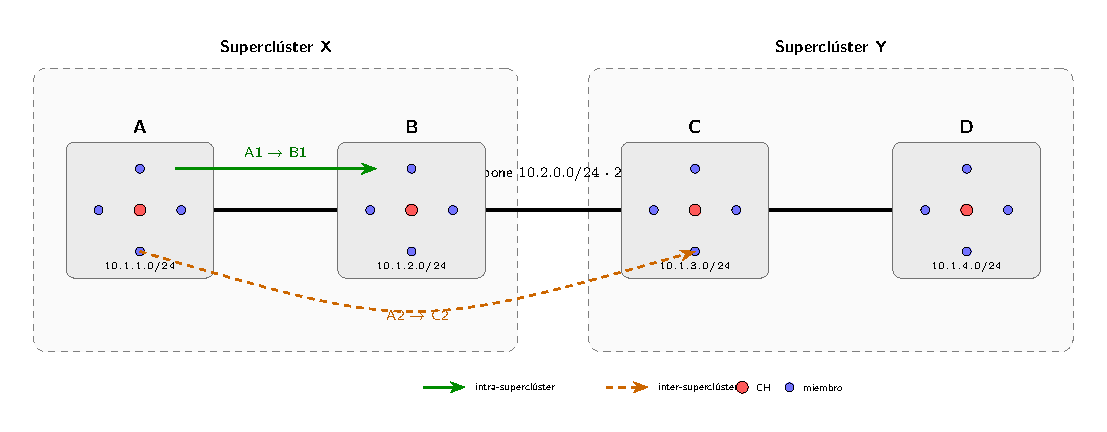
\includegraphics[width=0.95\textwidth]{Materiales/diagramas/arquitectura.pdf}
\caption{Arquitectura jerárquica de la MANET. Cada clúster tiene un canal WiFi ad hoc
independiente y una subred propia; los cuatro \emph{cluster heads} se comunican entre sí
por un canal \emph{backbone} compartido.}
\label{fig:diseno-arquitectura}
\end{figure}

La comunicación se separa en dos dominios. Dentro de cada clúster, los miembros y su CH
comparten un canal WiFi ad hoc independiente, de modo que un miembro solo puede hablar
directamente con los nodos de su propio clúster; no hay interferencia ni contienda entre
clústeres porque cada uno usa un canal distinto. Para que la información cruce de un
clúster a otro, los cuatro CH disponen de una segunda interfaz conectada a un canal
\emph{backbone} compartido, por el que se reenvía todo el tráfico interclúster. Esta
separación hace que el camino de un paquete entre miembros de clústeres distintos sea
siempre de la forma miembro $\rightarrow$ CH $\rightarrow$ \emph{backbone} $\rightarrow$
CH $\rightarrow$ miembro, lo que convierte a los enlaces entre CH en la columna vertebral
de la red.

El direccionamiento refuerza esa estructura: cada clúster es una subred propia
($10.1.1.0/24$ a $10.1.4.0/24$) y el \emph{backbone} es otra ($10.2.0.0/24$), de manera
que el enrutamiento distingue con claridad los saltos locales de los saltos
interclúster. Sobre todas las interfaces corre AODV, que al ser un protocolo reactivo
descubre las rutas a demanda y las repara cuando un enlace se rompe, exactamente el
mecanismo que el experimento quiere poner a prueba.

\subsection{Modelo de movilidad jerárquica}
\label{sec:diseno-movilidad}

El movimiento se modela en tres capas anidadas, en correspondencia con los niveles de la
jerarquía. Cada capa se desplaza \emph{relativa} a la capa que tiene por encima, de modo
que la posición absoluta de un nodo es la suma vectorial de las tres contribuciones:
\[
p(t) = p_S(t) + p_C(t) + p_N(t),
\]
donde $p_S(t)$ es la posición del centro del superclúster, $p_C(t)$ la del centro del
clúster respecto de su superclúster y $p_N(t)$ la del nodo respecto de su clúster. La
figura~\ref{fig:diseno-movilidad} representa esta composición.

\begin{figure}[h]
\centering
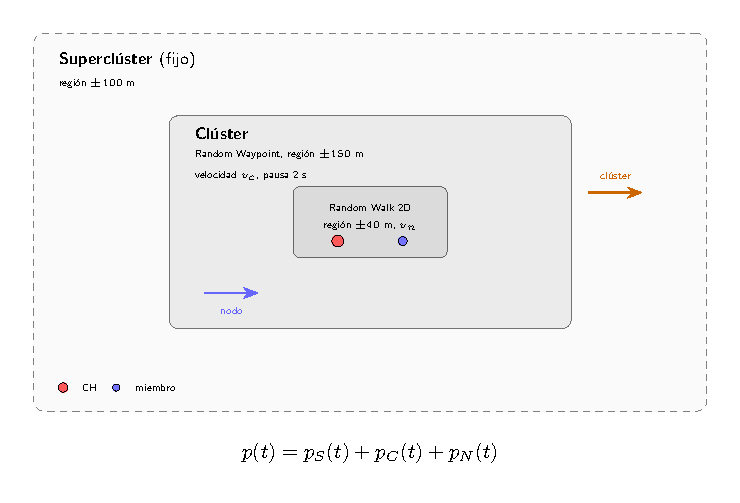
\includegraphics[width=0.9\textwidth]{Materiales/diagramas/movilidad.pdf}
\caption{Composición de la movilidad en tres capas. El clúster se mueve como un todo
dentro de su superclúster y, a su vez, cada nodo se mueve dentro de su clúster; la
posición final es la suma de las tres contribuciones.}
\label{fig:diseno-movilidad}
\end{figure}

Cada capa usa un modelo distinto, acorde con el papel que cumple. Los superclústeres
permanecen fijos en todos los experimentos, porque su única función es delimitar la
región en la que se mueven sus clústeres; el programa permite moverlos, pero el diseño
experimental deja su velocidad en cero. Los clústeres se mueven con un modelo
\emph{Random Waypoint} de velocidad constante dentro de una región de $\pm 150$\,m
alrededor del centro de su superclúster, con una pausa fija de 2\,s al llegar a cada
destino. Los nodos miembros se mueven con una caminata aleatoria bidimensional
(\emph{Random Walk 2D}) de velocidad constante dentro de una región de $\pm 40$\,m
alrededor del centro de su clúster, cambiando de rumbo cada 10\,m recorridos. El CH
permanece en el centro de su clúster. La tabla~\ref{tab:diseno-movilidad} resume las
capas.

\begin{table}[h]
\centering
\small
\begin{tabular}{llp{2.6cm}p{2.4cm}p{3.4cm}}
\toprule
\textbf{Capa} & \textbf{Modelo} & \textbf{Región} & \textbf{Velocidad} & \textbf{Observación} \\
\midrule
Superclúster & Fijo & $\pm 100$\,m & $v_S = 0$ & Solo organiza la jerarquía. \\
Clúster & Random Waypoint & $\pm 150$\,m & $v_C$ (constante) & Pausa de 2\,s entre destinos. \\
Nodo & Random Walk 2D & $\pm 40$\,m & $v_N$ (constante) & Cambia de rumbo cada 10\,m. \\
\bottomrule
\end{tabular}
\caption{Capas de movilidad y sus parámetros.}
\label{tab:diseno-movilidad}
\end{table}

La elección de modelos con velocidad constante es deliberada: en los escenarios E1 y E2
se mueve una sola capa a la misma velocidad $v$, lo que garantiza que ambos escenarios
sean comparables. La región de $\pm 40$\,m en que se mueven los nodos mantiene a un
miembro siempre a menos de 57\,m de su CH, dentro del alcance de 60\,m del canal del
clúster; la movilidad de nodo, por tanto, no puede desconectar a un miembro de su CH,
sino que solo altera la calidad de las rutas locales. La movilidad de clúster, en
cambio, sí puede alejar a dos CH más allá del alcance de 250\,m del \emph{backbone}, que
es precisamente el efecto que la hipótesis considera dominante.

\subsection{Flujo de la simulación}
\label{sec:diseno-flujo-simulacion}

El programa \texttt{manet-jerarquica.cc} sigue una secuencia lineal de fases, cada una
implementada en una función independiente. La figura~\ref{fig:diseno-flujo-simulacion}
muestra el orden y la correspondencia de cada fase con la parte del trabajo que la
construyó.

\begin{figure}[h]
\centering
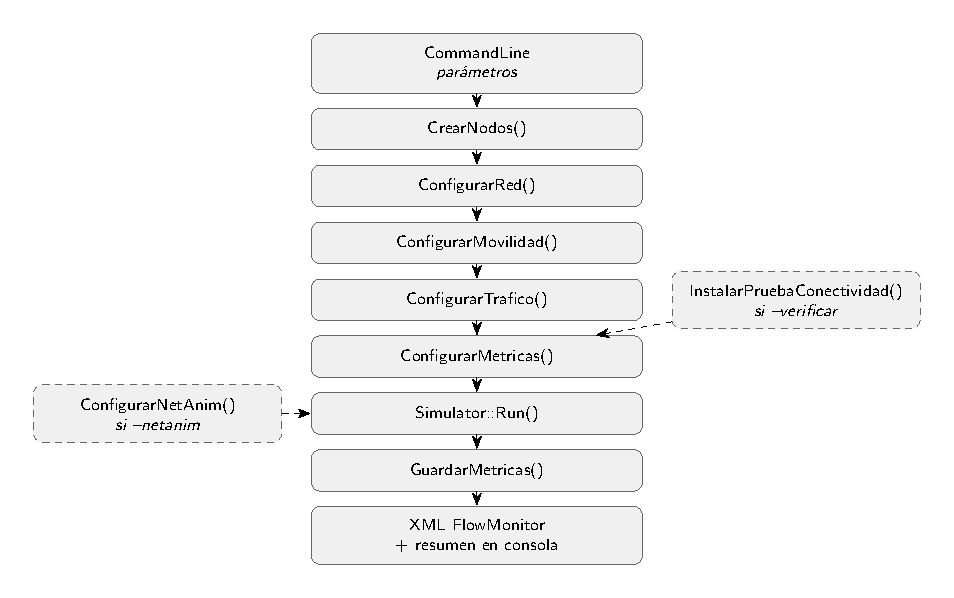
\includegraphics[width=0.85\textwidth]{Materiales/diagramas/flujo-simulacion.pdf}
\caption{Flujo de la simulación: los parámetros se leen, se crean los nodos y la red, se
configuran movilidad, tráfico y métricas, se ejecuta el simulador y se guardan los
resultados. Las ramas punteadas corresponden a los modos de verificación y de
visualización.}
\label{fig:diseno-flujo-simulacion}
\end{figure}

Primero se interpretan los parámetros de línea de comandos, que fijan el escenario, las
velocidades, la semilla y el directorio de salida. A continuación se crean los veinte
nodos y se los agrupa en clústeres y superclústeres; se instalan las interfaces WiFi con
sus canales y la pila IP con AODV; se configura la movilidad jerárquica; se inyectan los
ocho flujos de tráfico; y se instala el monitor de métricas. Solo entonces se ejecuta el
simulador y, al terminar, se serializan los resultados a XML y se imprime un resumen en
consola. Dos modos auxiliares completan el programa: con \texttt{--verificar} se corre
una prueba de conectividad entre clústeres y con \texttt{--netanim} se genera una traza
visual para NetAnim.

\newpage
El algoritmo que resume esa secuencia, independiente de la sintaxis de C++, se presenta
a continuación.

\begin{verbatim}
procedimiento Simular(escenario, v_cluster, v_nodo, semilla):
    leer parámetros y fijar la semilla
    crear 20 nodos
    agrupar en 4 clústeres (A-D) y 2 superclústeres (X, Y)

    para cada clúster:
        crear su canal WiFi propio (alcance 60 m)
        asignar la subred 10.1.k.0/24

    crear el canal backbone (alcance 250 m) para los 4 CH
    instalar la pila IP con AODV

    configurar la movilidad jerárquica:
        superclúster fijo
        clúster con Random Waypoint (±150 m, v_cluster)
        miembro con Random Walk 2D (±40 m, v_nodo)

    instalar 8 flujos UDP OnOff (puertos 5000-5007)
    instalar FlowMonitor
    ejecutar hasta T = 200 s
    guardar el XML de FlowMonitor y el resumen de métricas
\end{verbatim}

\subsection{Diseño experimental}
\label{sec:diseno-experimento}

Para responder la pregunta se comparan cuatro escenarios de movilidad: E0, sin
movimiento; E1, con solo movilidad de nodo; E2, con solo movilidad de clúster; y E3, con
ambas capas. Los escenarios con movimiento se evalúan a 1, 5, 10 y 20\,m/s, y cada
configuración se repite diez veces con semillas distintas, para un total de 130 corridas.
De cada corrida se obtienen la tasa de entrega, el retardo, el \emph{throughput} y el
\emph{jitter} a partir de los flujos de datos registrados por FlowMonitor. El análisis
compara las medias con intervalos de confianza del 95\,\% y contrasta E2 contra E1
mediante una prueba $t$ de Welch unilateral.

La comparación entre E1 y E2 es la que responde la pregunta de investigación. Como en
ambos se mueve una sola capa a la misma velocidad, la diferencia observada en la tasa de
entrega y en el retardo se puede atribuir al tipo de movilidad y no a un cambio en la
cantidad de movimiento. El escenario E3, que combina ambas capas, permite comprobar si
los efectos se acumulan cuando el movimiento ocurre en los dos niveles a la vez.

\subsection{Decisiones de diseño y su justificación}
\label{sec:diseno-decisiones}

Varias decisiones merecen justificarse explícitamente porque condicionan la
interpretación de los resultados. Se usaron cuatro clústeres en el nivel inferior, y no
tres, para que los dos superclústeres quedaran simétricos y los flujos pudieran
repartirse de forma equilibrada entre tráfico intra e inter-superclúster. Los
superclústeres se mantienen fijos para que, en cada escenario, se mueva una sola capa a
la velocidad de estudio; de otro modo no sería posible atribuir el efecto observado a un
tipo de movilidad concreto. La propagación se modela con un disco de alcance exacto, y
no con el modelo log-distancia por defecto de ns-3, porque con la potencia y el umbral
de detección estándar un enlace 802.11b a 1\,Mbps solo alcanza unos 50\,m, insuficiente
para sostener un \emph{backbone} entre clústeres separados 150\,m; el modelo de disco,
además, hace que la geometría sea fácil de controlar y de explicar. El tráfico se
distribuyó en ocho flujos de baja carga, cuatro dentro de cada superclúster y cuatro
entre superclústeres, para forzar el uso de la jerarquía sin saturar la red. Y se
descartó ns3-ai porque el problema no requiere aprendizaje ni control adaptativo: la
medición del efecto de la movilidad sobre AODV se resuelve de forma natural con la
simulación de eventos discretos de ns-3, y prescindir de capas adicionales reduce el
riesgo de incompatibilidades y acelera las corridas.
